
%(BEGIN_QUESTION)
% Copyright 2012, Tony R. Kuphaldt, released under the Creative Commons Attribution License (v 1.0)
% This means you may do almost anything with this work of mine, so long as you give me proper credit

An area at an oil refinery where high concentrations of toxic hydrogen sulfide (H$_{2}$S) gas exists in the process piping is equipped with a safety sensor switch to monitor ambient air for dangerous concentrations of H$_{2}$S gas.  A PLC receives the discrete signal from this switch, and the sensor itself is programmed with a ``trip'' point value to activate the discrete output any time the H$_{2}$S concentration in ambient air exceeds 8 parts per million (8 ppm):

$$\includegraphics[width=15.5cm]{i01884x01.eps}$$

The PLC program for this system is shown here:

$$\includegraphics[width=15.5cm]{i01884x02.eps}$$

Suppose the counter's accumulator value happens to be at a value of 4.  Now suppose the H$_{2}$S concentration jumps up from 1 ppm to 10 ppm stays there for 7 seconds before falling back down to 1 ppm.  Fifteen minutes of time go by, and then the H$_{2}$S concentration again jumps up to 10 ppm and this time remains that high for 21 seconds before dropping back down to 1 ppm.

\vskip 10pt

Identify the counter's accumulated value at the end of the 7-second gas event, and also at the end of the 21-second gas event.  Finally, identify whether or not the lamp will be energized at the end of the 21-second gas event.

\underbar{file i01884}
%(END_QUESTION)





%(BEGIN_ANSWER)

{\it 3 points for each correct accumulator value; 4 points for correct lamp status}

\vskip 10pt

The counter's accumulated value will be 5 at the end of the first gas event, and 6 at the end of the second gas event.  The lamp will remain de-energized the entire time.

%(END_ANSWER)





%(BEGIN_NOTES)

{\bf This question is intended for exams only and not worksheets!}.

%(END_NOTES)

